\documentclass[11pt]{article}
\usepackage[margin=1in]{geometry}
\usepackage{volfit_preamble}
\graphicspath{{figures/}}

\title{\textbf{Where the Likelihood Is Flat}\\[2pt]
\large Prior persistence as estimation in the flat directions of today's
data: yesterday may speak only where today is silent\\[2pt]
\normalsize Vol-Fitter Technical Notes, No.~13}
\author{Vol-Fitter}
\date{\today}

\begin{document}
\maketitle

% Generated numbers.  prior_flat_tables.tex carries everything unique to
% this edition (gen_prior_flat.py).  Never retype a generated number.
% Auto-generated by gen_prior_flat.py — do not edit.
\newcommand{\pflnfits}{8}
\newcommand{\pflspreadatmbp}{1}
\newcommand{\pflspreadwing}{2.6}
\newcommand{\pflnthin}{30}
\newcommand{\pflnout}{71}
\newcommand{\pflkptwofive}{-0.10}
\newcommand{\pflkctwofivereal}{0.06}
\newcommand{\pflkptwofivereal}{-0.08}
\newcommand{\pflopwingerr}{0.0}
\newcommand{\pflsgwingerr}{0.7}
\newcommand{\pflsgoldgap}{3.3}
\newcommand{\pflopwingerrdeep}{0.3}
\newcommand{\pflsgwingerrdeep}{3.7}
\newcommand{\pflatmopgap}{0.00}
\newcommand{\pflatmfacgap}{0.00}
\newcommand{\pfljump}{4}
\newcommand{\pflunmet}{48}
\newcommand{\pflnsparse}{5}
\newcommand{\pflgapdenseatm}{0.00}
\newcommand{\pflgapsparseatm}{0.00}
\newcommand{\pflgapdenserr}{0.00}
\newcommand{\pflgapsparserr}{0.00}
\newcommand{\pflgapdensebf}{0.00}
\newcommand{\pflgapsparsebf}{0.00}
\newcommand{\pflgapdensevs}{0.00}
\newcommand{\pflgapsparsevs}{0.57}
\newcommand{\pfltaildeltas}{2/5/10}
\newcommand{\pflbtnodes}{1116}
\newcommand{\pflhybimpr}{32}
\newcommand{\pflhybwin}{66}
\newcommand{\pflsgimpr}{28}
\newcommand{\pflsgwin}{63}
\newcommand{\pflopwin}{30}
\newcommand{\pflfacwin}{34}
\newcommand{\pflspybandrms}{2}
\newcommand{\pflspywingmo}{90}
\newcommand{\pflspywinghy}{42}
\newcommand{\pflrefagree}{\ensuremath{1.0\times10^{-17}}}
\newcommand{\pflgencommit}{652da29}
\newcommand{\pflgendate}{2026-07-19}


\begin{abstract}
A sparse morning does not determine a smile.  On a real SPY expiry with
quotes confined to the at-the-money band, \pflnfits\ production
calibrations agree to \pflspreadatmbp\ vol bp where quoted and disagree
by \pflspreadwing\ vol points at $k=-0.30$: the likelihood has flat
directions, and something other than the data must choose along them.
This lecture develops the Vol-Fitter's prior persistence as the answer
to exactly that question.  Yesterday's surface enters today's fit as
extra least-squares rows, but a row is admitted only where today's
quotes fail to identify its coordinate: an \emph{activation gate} with
a provable dead zone (a well-observed coordinate receives exactly zero
prior weight, not a small one), an information price for every
persisted quantity (the precision of a signed basket is the harmonic
combination of its legs' quote support --- one dead leg unidentifies
the basket), and a choice of coordinates that keeps yesterday out of
what today has measured (risk-reversals and butterflies annihilate the
level direction that per-strike anchoring damps).  The same
principle in coverage currency gives the strike-gap anchor, whose
absolute-price rows are right when the level is stable and wrong
across a jump --- measured here on a controlled \pfljump-point
overnight jump, where the operator rows reconstruct the lifted wing to
\pflopwingerrdeep\ vol points while the strike anchor misses it by
\pflsgwingerrdeep.  We also prosecute the gate's own blind spot: its
support proxy credits identification one kernel bandwidth beyond the
last quote, which closes every vol-operator gate on a liquid morning
--- the measured reason the pure operator modes add nothing at the
median of the stored \pflbtnodes-node temporal backtest, while the
shipped hybrid default (shape operators plus deep-tail strike anchors)
improves held-out wing reconstruction by $\sim$\pflhybimpr\ vol bp,
\pflhybwin\% of the time.  On the running SPY node the hybrid refit
holds the retained band to \pflspybandrms\ vol bp while reconstructing
the withheld wing to \pflspywinghy\ vol bp rms against the market-only
fit's \pflspywingmo.
\end{abstract}

\newpage
\tableofcontents
\newpage

%======================================================================
\section{The morning after}
\label{sec:flat}

Overnight, two things change unevenly.  The at-the-money level moves on
fresh news and is immediately re-quoted; the wings may receive no
fresh quote at all, yet the book still needs values there.  The naive
alternatives both fail in known ways: refit today's quotes alone and
the unconstrained wings \emph{flap}; anchor the whole fit to
yesterday and the prior \emph{damps} the genuine at-the-money move.
Before designing anything, it pays to say precisely what a sparse
morning leaves undetermined.

\Cref{fig:flat} does this on the note's running character --- a real
SPY expiry (December 2026) from a live production export, its
\pflnthin\ morning quotes confined to $|k|\le0.10$.  We fit the band
\pflnfits\ times with production calibrators: one model family at
three resolutions and two regularization strengths, plus two entirely
different parametric families.  Panel~A shows all eight: on the quoted
band they are one curve (maximum disagreement \pflspreadatmbp\ vol bp);
at $k=-0.30$ they disagree by \pflspreadwing\ vol points.  The
likelihood --- the weighted sum of squared quote residuals, whatever
the model --- is \emph{flat} along the directions that move the wings
while leaving the band unchanged, and every fitter must pick a point
on that flat set by some rule: a regularizer, a parametric family's
built-in tail habit, a prior.  Panel~B quantifies where the flatness
lives: the effective quote count $s(k)$ (defined in \cref{sec:info})
collapses outside the band exactly where the ensemble spread opens.

\begin{figure}[H]
\centering
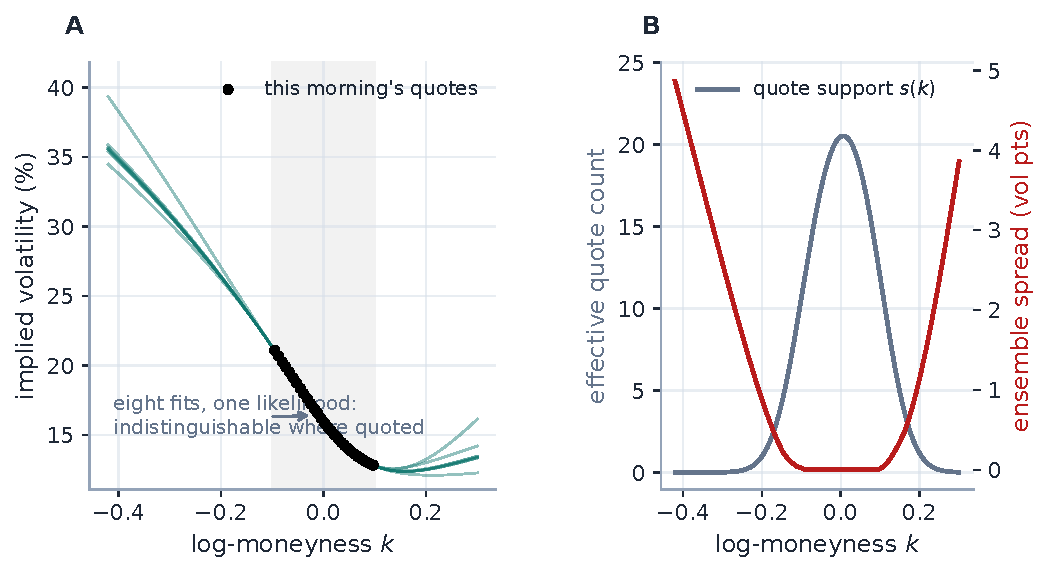
\includegraphics[width=\textwidth]{fig_pfl_flat.pdf}
\caption{What a sparse morning does not determine (real SPY node,
production calibrators).  A: \pflnfits\ fits --- one family at several
resolutions and regularizations, plus two other model families ---
agree to \pflspreadatmbp\ vol bp on the quoted band (shaded) and spread
\pflspreadwing\ vol points at $k=-0.30$.  The data does not choose; the
extrapolation rule does.  B: the quote-support profile $s(k)$ (left
axis) collapses precisely where the ensemble spread (right axis)
opens: flatness is measurable, coordinate by coordinate.}
\label{fig:flat}
\end{figure}

The design question of this note is therefore \emph{not} ``how hard
should the prior pull?''\ but ``\emph{where} is the prior allowed to
pull at all?''  The answer the fitter ships: only along the flat
directions.  A feature today's quotes identify belongs to today; a
feature they do not belongs to yesterday, transported to today's
market.  Damping is what happens when the prior leaks into the
identified directions; flapping is what happens when nothing occupies
the unidentified ones.

\begin{invariant}
\begin{enumerate}[leftmargin=1.6em]
\item \textbf{Do not damp the signal.}  A coordinate today's quotes
identify at the required precision receives prior weight exactly zero
--- a dead zone, not a small bias.
\item \textbf{Fill the gap.}  A coordinate today's quotes do not
identify is held at the transported prior, with strength growing as
coverage falls.
\item \textbf{Strictly additive.}  Mode \texttt{off} is byte-identical
to a plain fit; every prior block is a no-op when its target is empty.
\item \textbf{Coupled features persist coupled.}  A risk-reversal is
one statement about the smile, not two statements about strikes;
persistence must not silently decompose it.
\end{enumerate}
\end{invariant}

\paragraph{Conventions and the notation ledger.}
One time symbol: $\tau$, the node's variance time (Note~11 owns the
clock question; every prior value below is re-expressed at the node's
$\tau$, and the rescale cancels in vol space).  Subscripted $\partial$
for the rare partial derivative; primes are never used.  One move
symbol: $h=\log(F_{\text{now}}/F_{\text{prior}})$, reserved for the
transported forward distance.  One bandwidth symbol: $b$, the Gaussian
kernel width of the support measure \emph{and} the factor stencil step
--- production deliberately ties both to a single knob.

\begin{table}[H]
\centering\footnotesize
\setlength{\tabcolsep}{3pt}
\begin{tabular}{@{}llll@{}}
\toprule
$k,\ \tau$ & log-moneyness; variance time &
$\sigma(k),\ w(k)=\sigma^2\tau$ & implied vol; total variance\\[2pt]
$O=c\T\sigma=\sum_a c_a\sigma(k_a)$ & a signed basket over legs $k_a$ &
$s_a,\ s(k),\ b$ & quote support; its bandwidth\\[2pt]
$\pi,\ \pi_{\mathrm{req}}$ & observation precision; requirement &
$g,\ \gamma$ & the activation gate; its exponent\\[2pt]
$\lambda_j,\ B$ & row weight; a mode's budget &
$\rho_{\mathrm{obs}},\rho_{\mathrm{des}},\Delta x_j,u$ & densities;
cell width; unmet fraction\\[2pt]
$h$ & transported forward move &
$\Delta,\ \1$ & option delta; the level direction\\
\bottomrule
\end{tabular}
\caption{Every symbol in the note.  Nothing is reused with a second
meaning; $b$ is one symbol because production makes it one knob.}
\label{tab:ledger}
\end{table}

%======================================================================
\section{Yesterday as evidence: the Bayesian rows}
\label{sec:rows}

The mechanics are ordinary Bayesian least squares.  Yesterday's
surface, transported to today's forward (\cref{sec:transport}),
supplies \emph{pseudo-observations}: functionals $O_j$ evaluated on
the prior become targets for the same functionals evaluated on the
model, appended to the data rows.  Every persistence mode in the
fitter --- strike anchors, quote operators, smile factors --- adds
rows of one universal shape,
\begin{equation}
\boxed{\;r_j=\sqrt{\lambda_j}\;
\frac{O_j(\theta)-O_j(\text{prior})}{\text{scale}_j},\;}
\label{eq:universal}
\end{equation}
where $O_j$ is a call price at a delta location, a quote operator
(ATM, risk-reversal, butterfly, var-swap), or a local smile factor,
depending on the mode (\cref{sec:modes}), and $\theta$ is whichever
model is being calibrated --- the rows are model-agnostic because they
only consult the model's smile.

Everything therefore reduces to choosing the weights $\lambda_j$.  For
one scalar coordinate the posterior is the precision-weighted average:
a datum $d$ at precision $\pi$ against a prior mean $\mu$ at precision
$\lambda$ gives posterior mean $(\lambda\mu+\pi d)/(\lambda+\pi)$, so
the \emph{share of the posterior owned by the prior} is
$\lambda/(\lambda+\pi)$.  Here is the first design fork.  A
\emph{ridge} --- fixed $\lambda>0$, however small --- owns a positive
share of every coordinate: it biases the well-observed ATM exactly as
surely as it stabilizes the dark wing, only less.  Under invariant~1
that is not a small flaw but a disqualification: no fixed prior
precision has a dead zone.  The prior precision must depend on the
data.

\begin{definition}[Activation gate]
\label{def:gate}
For observation precision $\pi\ge0$, required precision
$\pi_{\mathrm{req}}>0$ and sharpness $\gamma>0$,
\begin{equation}
g(\pi)=\Big(\min\big(\max\big(1-\pi/\pi_{\mathrm{req}},\,0\big),
\,1\big)\Big)^{\gamma}.
\label{eq:gate}
\end{equation}
\end{definition}

The gate is $1$ where the data says nothing, decreases monotonically
as the data improves, and --- the decisive property --- is
\emph{exactly zero} for all $\pi\ge\pi_{\mathrm{req}}$, not
asymptotically small.  $\gamma$ sharpens the edge.  The prior
precision actually entering the fit is $\lambda\,g(\pi)$, and
\cref{fig:gate}B shows the resulting posterior share against the
ridge's: same behaviour in the dark, a hard zero in the light.

\begin{proposition}[The no-damp guarantee]
\label{prop:nodamp}
Fix a mode and let coordinate $j$ satisfy
$\pi_j\ge\pi_{\mathrm{req},j}$, so $g_j=0$ and hence $\lambda_j=0$ in
\eqref{eq:universal}.  Then $r_j\equiv0$ for every parameter vector
$\theta$: the objective, its gradient and its Gauss--Newton model are
independent of the prior value $O_j(\text{prior})$.  In particular,
with all gates closed the fit is the prior-free fit, and with mode
\texttt{off} the fit is byte-identical to a plain fit.
\end{proposition}

\begin{proof}
$\lambda_j=0$ makes $r_j$ the zero function of $\theta$: it
contributes $0$ to the cost and a zero row to the Jacobian, so nothing
downstream can depend on the prior through it.  The byte-identity
claims are locked by
\texttt{test\_none\_anchor\_leaves\_the\_fit\_byte\_identical} and the
\texttt{off}-mode routing tests (\cref{app:trace}).
\end{proof}

This is the difference between gating and shrinkage, and it is worth
naming in the standard vocabulary: Tikhonov regularization
\cite{Tikhonov1977} stabilizes by biasing everywhere; the gate is a
data-dependent penalty whose support is confined to the coordinates
the data left unidentified.  It spends its entire budget where the
likelihood is flat and nothing anywhere else.

\begin{lstlisting}[caption={The activation gate \eqref{eq:gate},
verbatim from the shared vocabulary (\texttt{calib/precision.py});
executed against production in \cref{app:ref}.},label={lst:gate}]
def activation_gap(obs, req, gamma=1.0):  # 1: data silent; 0: identified
    return np.clip(1 - obs/np.maximum(req, 1e-12), 0.0, 1.0)**gamma
\end{lstlisting}

\begin{figure}[H]
\centering
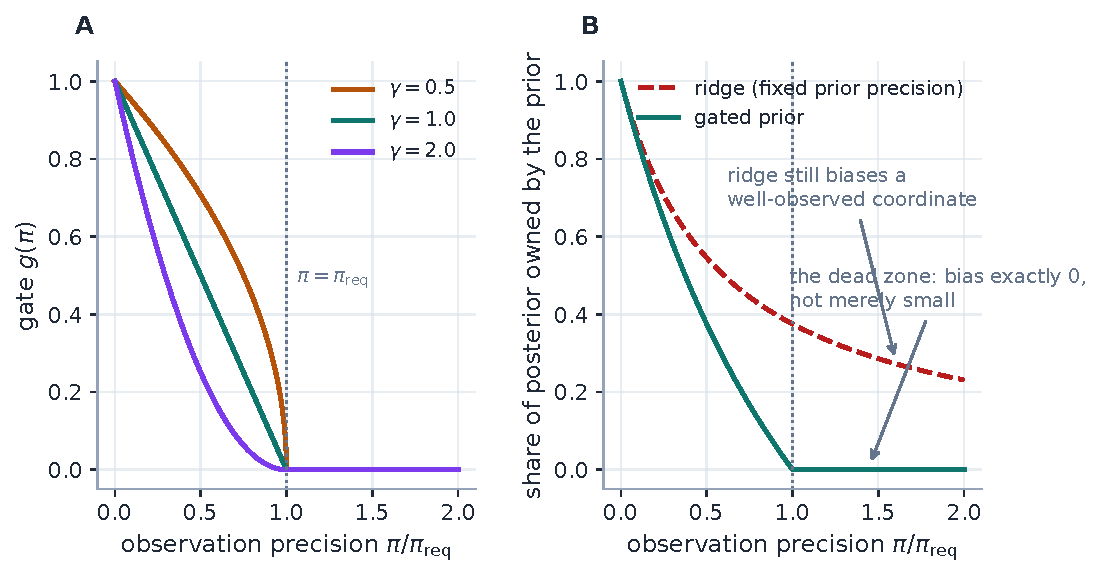
\includegraphics[width=\textwidth]{fig_pfl_gate.pdf}
\caption{The gate and why shrinkage cannot replace it (production
\texttt{activation\_gap}).  A: the gate \eqref{eq:gate} for three
sharpness values --- past the required precision the prior weight is
exactly zero.  B: the share of the posterior owned by the prior.  A
ridge with fixed prior precision (dashed) still owns a quarter of a
coordinate observed at twice the requirement; the gated prior (solid)
owns exactly nothing --- the dead zone that turns ``do not damp the
signal'' from a preference into a theorem.}
\label{fig:gate}
\end{figure}

\paragraph{Exercise 1.}
Show that under a fixed-precision ridge the posterior bias of a
coordinate with true value $d$ and prior mean $\mu$ is
$(\mu-d)\,\lambda/(\lambda+\pi)$, and that requiring this to vanish
for all well-observed coordinates while keeping $\lambda>0$ for
unobserved ones forces $\lambda$ to depend on $\pi$ with a zero at
finite $\pi$ --- i.e.\ forces a gate of the form \eqref{eq:gate} up to
the choice of the descent profile.

%======================================================================
\section{Measuring flatness: the information of a functional}
\label{sec:info}

The gate consumes a precision $\pi$; the fitter must produce one per
persisted coordinate, cheaply, before fitting.  The shipped currency
is \emph{quote support}: each leg location $k_a$ receives the
Gaussian-kernel effective quote count
\begin{equation}
s_a=\sum_q \tilde\omega_q\,
e^{-(k_q-k_a)^2/2b^2},
\label{eq:support}
\end{equation}
with $k_q$ the live quote locations, $\tilde\omega_q$ the fit weights
normalized to mean one (so $s_a$ reads as ``how many quotes
effectively sit on this leg'' under any weighting scheme), and $b$ the
bandwidth.  A quote exactly on the leg contributes one; a quote a few
bandwidths away contributes nothing.

Support prices a \emph{leg}.  The persisted objects are
\emph{baskets} $O=c\T\sigma$ over several legs, and their price
follows from the standard sampling theory of a linear functional
\cite{LehmannCasella1998}:

\begin{assumption}
\label{ass:diag}
Each leg vol is estimable from today's quotes with variance
proportional to $1/s_a$, independently across legs (a diagonal
information model; \cref{sec:blind} examines where it fails).
\end{assumption}

\begin{proposition}[Harmonic support is the propagated basket precision]
\label{prop:harmonic}
Under \cref{ass:diag}, the implied estimate of $O=\sum_a c_a\sigma(k_a)$
has variance proportional to $\sum_a c_a^2/s_a$, i.e.\ precision
\begin{equation}
\pi(O)=\Big(\sum_a\frac{c_a^2}{s_a+\eps}\Big)^{-1}.
\label{eq:harmonic}
\end{equation}
In particular one unquoted leg ($s_a\to0$) drives $\pi(O)\to0$
however well the other legs are quoted: a risk-reversal with a
missing put leg is unidentified, and its gate opens.
\end{proposition}

\begin{proof}
$\Var\big(\sum_ac_a\hat\sigma_a\big)=\sum_ac_a^2\Var(\hat\sigma_a)
\propto\sum_ac_a^2/s_a$ by independence; take reciprocals.  The
$\eps$ regularizes the empty-leg limit.
\end{proof}

\Cref{fig:basket} shows both faces of \eqref{eq:harmonic} computed by
the production builder.  Panel~A sweeps a widening quote band on a
controlled smile: the ATM basket is identified almost immediately,
while the risk-reversal and butterfly stay dark until the band
approaches their $25\Delta$ legs --- and begin to rise \emph{one
bandwidth before} the quotes actually arrive, the kernel bleed we
prosecute in \cref{sec:blind}.  Panel~B is the dead-leg law: with the
call leg well quoted, the basket precision still collapses linearly as
the put leg's support vanishes.

\begin{figure}[H]
\centering
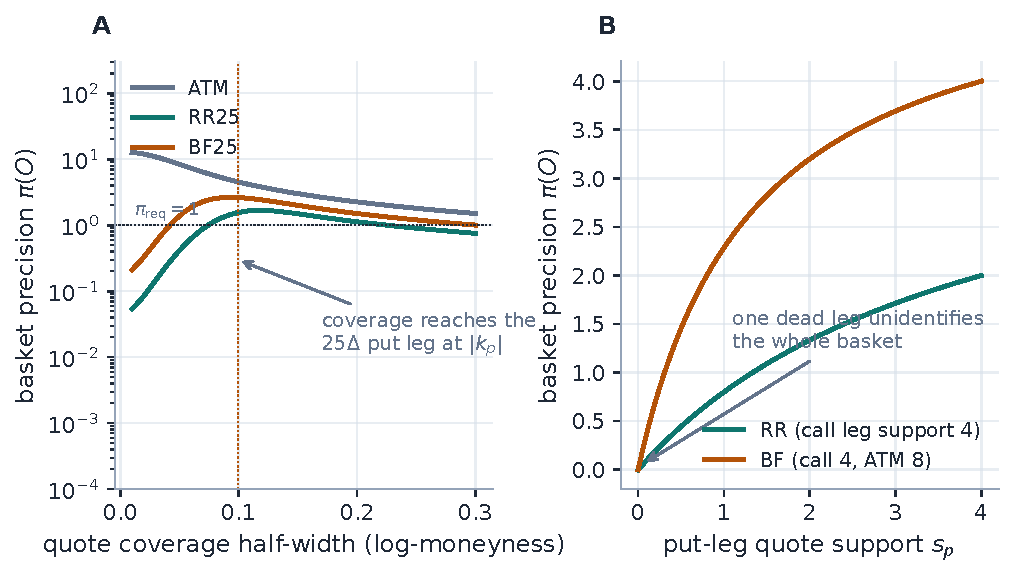
\includegraphics[width=\textwidth]{fig_pfl_basket.pdf}
\caption{The information price of a basket (production support and
gate machinery).  A: precision of ATM, RR25 and BF25 as a fixed budget
of quotes spreads over a widening band --- the wing baskets cross the
requirement (dotted) only when coverage approaches the $25\Delta$ put
leg (vertical line), and decline again as the same quotes thin out.
B: one dead leg unidentifies the whole basket, however well the others
are quoted --- the harmonic law \eqref{eq:harmonic}.}
\label{fig:basket}
\end{figure}

\begin{remark}[Identifiability belongs to the functional, not the legs]
\label{rem:bfrr}
Take symmetric wing support $s_c=s_p=s$ and abundant ATM support.
Then $\pi(\text{RR})=s/2$ but
$\pi(\text{BF})\approx2s$: the butterfly's wing coefficients of
$\tfrac12$ enter \eqref{eq:harmonic} squared, so \emph{the same legs}
make the butterfly four times easier to identify than the
risk-reversal.  This is visible in production: on the case-file market
of \cref{sec:coords} the gate closes BF25 while leaving RR25 open
(\cref{fig:activation}B) --- the budget concentrates on the one shape
coordinate the morning genuinely left dark.
\end{remark}

The active weights split a mode's budget over the open gates,
\begin{equation}
\lambda_j=B\,\frac{g_j}{\sum_i g_i},
\qquad B=\frac{\text{strength}\,\%}{100}\sum_q\omega_q ,
\label{eq:budget}
\end{equation}
and operators with $g_j=0$ are dropped from the target entirely ---
they never reach the optimizer.  Making the budget a percentage of the
summed quote weights keeps the prior's strength proportional to how
much evidence the fit actually has.

\begin{remark}[What the shipped gate does \emph{not} use]
\label{rem:notused}
The requirement $\pi_{\mathrm{req}}$ is one scalar for all operators
(a per-operator schedule is declared in the design but not
implemented), and the split \eqref{eq:budget} does \emph{not} multiply
a base prior precision.  The richer vocabulary that lives beside the
gate in \texttt{calib/precision.py} --- the scalar confidence factors
\begin{equation}
\begin{aligned}
\text{density}&=\mathrm{clip}(n/8,\,0.15,\,1), &
\text{spread}&=\frac{1}{1+\text{rel spread}/0.05},\\
\text{freshness}&=2^{-\text{age}/\text{half-life}}
\ (3\,\text{d obs},\ 30\,\text{d prior}), &
\text{transport}&=e^{-|h|/0.10},
\end{aligned}
\label{eq:factors}
\end{equation}
plus fit quality $1/\text{rms}^2$ floored at one vol bp and
\texttt{active\_prior\_precision} --- is consumed by the \emph{graph
baseline} of Note~14, which imports these functions from here.  The
re-export is golden-locked, so the persistence gate and the graph
price identifiability in one language and cannot silently drift apart.
\end{remark}

\paragraph{Exercise 2.}
A risk-reversal has call-leg support $s_c=6$ and put-leg support
$s_p=0.1$.  Compute $\pi(\text{RR})$ from \eqref{eq:harmonic}
($\approx0.098$: the gate is nearly fully open at
$\pi_{\mathrm{req}}=1$), then let $s_p\to0$ and confirm the basket is
unidentified regardless of $s_c$.  Repeat for the butterfly with
abundant ATM support and conclude the factor-of-four of
\cref{rem:bfrr}.

%======================================================================
\section{Choosing coordinates: why baskets}
\label{sec:coords}

The gate acts coordinate by coordinate.  That makes the \emph{choice
of coordinates} load-bearing: gating can only keep yesterday out of
what today has measured if ``measured'' and ``unmeasured'' land in
different coordinates.  The smile's natural trader coordinates do
exactly this, and the fitter persists them directly.

\begin{definition}[Quote operators]
\label{def:operators}
With $\sigma(k)$ a slice's implied vol, $k_{c,\delta},k_{p,\delta}$
the call/put strikes at delta $\delta$ located on the \emph{prior}
smile and frozen, and \texttt{collarSign} fixing the orientation:
\[
\text{ATM}=\sigma(0),\qquad
\text{RR}_\delta=\pm\big(\sigma(k_{c,\delta})-\sigma(k_{p,\delta})\big),\qquad
\text{BF}_\delta=\tfrac12\big(\sigma(k_{c,\delta})
+\sigma(k_{p,\delta})\big)-\sigma(0),
\]
plus $\text{VarSwap}=\sqrt{K_{\mathrm{var}}/\tau}$ by log-contract
replication.  Each is a signed basket $O=c\T\sigma$; the registry
knows $\{$ATM, RR25, BF25, RR10, BF10, VarSwap$\}$.  Because the legs
are frozen on the transported prior, prior and model are compared at
the same log-moneyness, and the variance-time rescale between the
prior's clock and the node's cancels in vol space --- what persists is
the \emph{shape}, not the variance.
\end{definition}

\begin{definition}[Smile factors]
\label{def:factors}
The factor mode replaces delta legs by ATM-local stencils of step $b$:
$\text{skew}=\sigma(b)-\sigma(-b)$,
$\text{curvature}=\sigma(b)-2\sigma(0)+\sigma(-b)$,
$\text{leftWing}=\sigma(-3b)-\sigma(0)$,
$\text{rightWing}=\sigma(3b)-\sigma(0)$ --- raw differences, not
divided by the step, so they remain vol-magnitude quantities
comparable to the level, and prior and model use the same stencil.
Factors are structurally identical baskets and reuse the operator
gate, budget split and target machinery verbatim; they bite on
genuinely sparse smiles, where even the local shape is dark.
\end{definition}

Why baskets and not legs?  Because the coordinates decide what the
penalty can damp.

\begin{proposition}[Baskets annihilate exactly the directions legs
would damp]
\label{prop:nullspace}
Consider one operator $O=c\T\sigma$ over $L$ legs and compare two
penalties on the leg vols $\sigma\in\R^L$: the basket row
$r_{\mathrm{bsk}}=\sqrt\lambda\,(c\T\sigma-c\T\sigma^{\mathrm{prior}})$
and the per-leg stack
$r_a=\sqrt{\lambda_a}\,(\sigma_a-\sigma_a^{\mathrm{prior}})$,
$a=1,\dots,L$.  The basket penalty is invariant under every move
$\delta$ with $c\T\delta=0$ --- an $(L{-}1)$-dimensional space that,
for RR and BF, contains the common level shift $\delta=\1$, since
their coefficients sum to zero.  The per-leg stack is invariant only
under $\delta=0$: at $\sigma^{\mathrm{prior}}+t\1$ its cost grows as
$t^2\sum_a\lambda_a$, i.e.\ it damps a market-wide vol move even when
the market's RR and BF are unchanged.
\end{proposition}

\begin{proof}
$r_{\mathrm{bsk}}$ depends on $\sigma$ only through $c\T\sigma$, so
its level sets are affine hyperplanes with normal $c$; any
$\delta\in c^{\perp}$ leaves it fixed and $\dim c^{\perp}=L-1$.  For
RR, $c=(+1,-1)$; for BF, $c=(\tfrac12,\tfrac12,-1)$; both satisfy
$c\T\1=0$, so $\1\in c^{\perp}$.  The per-leg stack has Jacobian
$\diag(\sqrt{\lambda_a})$ of full rank, so its only invariant
direction is $0$, and its value at $\sigma^{\mathrm{prior}}+t\1$ is
$t^2\sum_a\lambda_a$.
\end{proof}

This is invariant~4 made precise, and it is the theorem behind a
design reversal.  The first local-volatility route emitted synthetic
\emph{per-leg} quotes at the operator legs --- and silently damped the
level, exactly as the proposition predicts.  The shipped design emits
one signed basket per operator; on the local-vol surface, where the
natural unknowns are call prices, the basket is transported to price
space by the frozen-vega linearization
$\sigma(k_a)\approx\sigma^{\mathrm{prior}}_a
+(P_a-P^{\mathrm{prior}}_a)/\text{vega}_a$: weights
$c_a/\text{vega}_a$, target $\sum_a(c_a/\text{vega}_a)
P^{\mathrm{prior}}_a$, tolerance $1/\sqrt\lambda$.  The same reform
cured a long-standing asymmetry: the SVI and Multi-Core Sigmoid
overlays, which previously received no prior at all, consume the same
operator targets as the LQD path --- one target, every model.

\Cref{fig:level} runs the whole argument through the production
calibrator on a controlled experiment: yesterday's smile, today's
truth the \emph{same shape lifted by \pfljump\ vol points}, quotes
only at the money.  The operator rows (which cannot see the level)
ride today's quotes and reconstruct the lifted wing to
\pflopwingerrdeep\ vol points at $k=-0.20$; the per-strike price
anchors of \cref{sec:coverage} cling to yesterday's absolute wing ---
\pflsgwingerrdeep\ vol points below today's truth, and only
\pflsgoldgap\ from yesterday's un-jumped curve.  Meanwhile the
at-the-money fit under the operator prior matches the data-only fit to
\pflatmopgap\ vol points (factors: \pflatmfacgap) --- the dead zone
holding in a live calibration.

\begin{figure}[H]
\centering
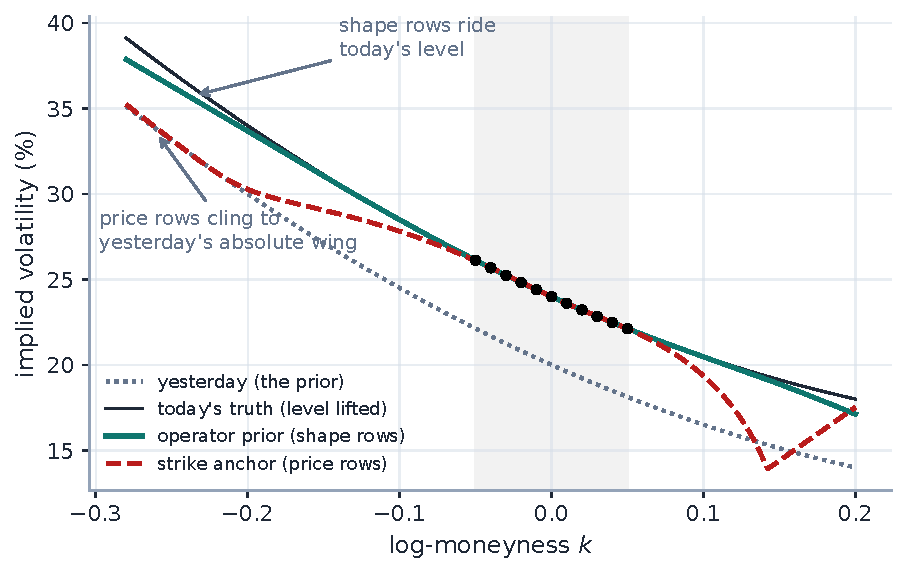
\includegraphics[width=0.9\textwidth]{fig_pfl_level.pdf}
\caption{Coordinates decide what gets damped (production calibrator, a
controlled \pfljump-point overnight level jump, quotes only in the
shaded band).  The operator prior --- shape baskets that annihilate
the level direction (\cref{prop:nullspace}) --- rides today's level
and lands on the lifted truth; the strike anchor --- absolute price
rows --- pins the unquoted wing to yesterday's curve.  The kink in the
strike-anchor fit on the call side is the same cling on the other
wing, where the anchors pull below today's smile.}
\label{fig:level}
\end{figure}

\paragraph{Exercise 3.}
For the RR pair $c=(+1,-1)$ verify $\1\in c^{\perp}$ and compute the
per-leg penalty of the level shift $t\1$ at weights
$\lambda_1=\lambda_2=\lambda$: cost $2\lambda t^2$, gradient
$2\lambda t$ per leg --- a restoring force toward yesterday's level
proportional to the jump.  With $t=\pfljump$ vol points and the
case-file budget this is the entire damping measured in
\cref{fig:level}; the basket penalty's force along $\1$ is
identically zero.

%======================================================================
\section{The same principle in coverage currency}
\label{sec:coverage}

The strike-gap mode is the older mechanism, and it answers the same
question --- where may the prior pull? --- with a different
measurement.  Instead of pricing the precision of a functional, it
measures a \emph{density deficit} in strike space.  With
$\rho_{\mathrm{obs}}$ the Gaussian kernel density of today's quote
locations (total mass the quote count, bandwidth $0.06$) and
$\rho_{\mathrm{des}}$ a desired coverage of the same mass spread over
the wider anchor span (uniform, or shaped by the prior's time value),
each anchor strike $x_j$ --- placed at the deltas
$\{2,5,10,25,40\}\Delta$ through the Black delta map
$k=\tfrac12\sigma^2\tau-\sigma\sqrt\tau\,\Phi^{-1}(c)$, with $\sigma$
resolved locally by a two-step fixed point --- receives
\begin{equation}
\text{weight}_j
=B_{\mathrm{sg}}\,
\frac{\big(\rho_{\mathrm{des}}(x_j)-\rho_{\mathrm{obs}}(x_j)\big)^{+}
\,\Delta x_j}
{\sum_i\big(\rho_{\mathrm{des}}(x_i)-\rho_{\mathrm{obs}}(x_i)\big)^{+}
\,\Delta x_i},
\qquad
u=\frac{\sum_i(\cdots)^{+}\,\Delta x_i}{\text{desired mass}},
\label{eq:deficit}
\end{equation}
with $\Delta x_j$ the anchor's Voronoi cell width, so each weight is
the missing quote mass in its cell.  The residual is the
vega-normalized \emph{call-price} difference at $x_j$ --- the same
form as the data block, so it reads as a vol error --- with the
deep-wing $1/\text{vega}$ capped at $25\times$ its minimum so a
vanishing tail vega cannot let one anchor amplify noise unboundedly.
Where quotes already meet the desired density the deficit is zero:
the same ``off where the data speaks'' behaviour as \cref{def:gate},
expressed as coverage rather than precision, and never multiplied by
a prior confidence.  The companion var-swap pull is scaled by the
unmet fraction $u$: a fully covered smile persists nothing, including
its var-swap level.  On the running SPY morning,
$u=\pflunmet\%$ --- half the desired coverage is missing, all of it
in the wings, and \cref{fig:activation}A shows the budget landing
exactly there.

\begin{caution}
The two mechanisms persist different \emph{things}.  Strike-gap rows
anchor absolute call prices: if the whole vol level jumps overnight,
an unquoted wing is pulled toward yesterday's \emph{absolute} wing ---
correct when the level is stable, wrong across a jump
(\cref{fig:level}, measured: \pflsgwingerrdeep\ vol points of miss).
Operator and factor rows anchor level-invariant shape --- RR, BF,
curvature are unchanged by $\sigma\mapsto\sigma+c$ --- so the
persisted wing rides today's level.  This is why the shipped default
carries the shape on operators and reserves strike anchors for the
deep tail no operator covers (\cref{sec:modes}).
\end{caution}

\begin{figure}[H]
\centering
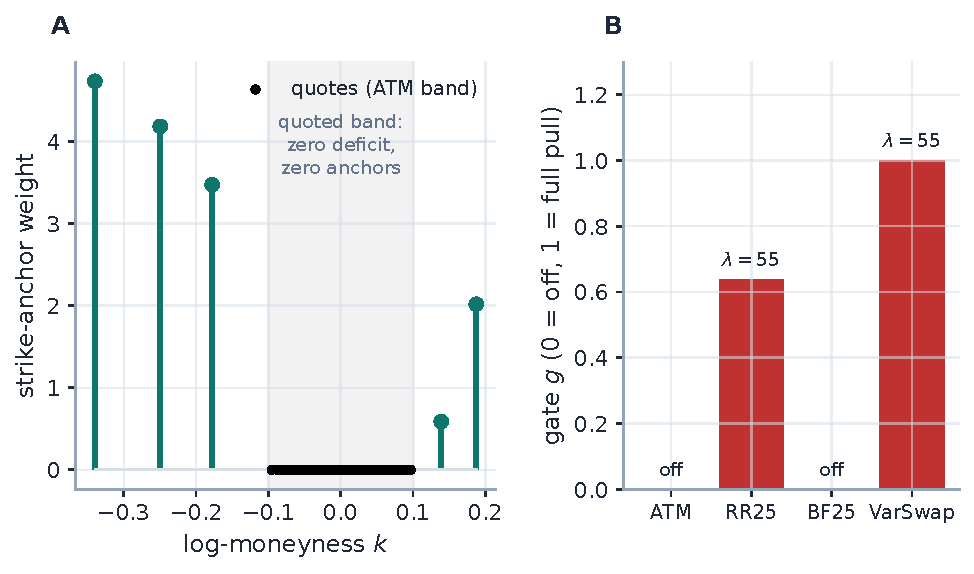
\includegraphics[width=\textwidth]{fig_pfl_activation.pdf}
\caption{Both mechanisms placing their budget, computed by the
production builders.  A: the strike-gap deficit \eqref{eq:deficit} on
the running SPY morning --- anchors inside the quoted band get zero
budget; the deep put anchors get most of it (unmet fraction
\pflunmet\%).  B: the operator gate on the case-file jump market ---
ATM is identified (gate closed, dropped from the target), the
butterfly is closed by its easier information price
(\cref{rem:bfrr}), and the budget concentrates on the open
risk-reversal and var-swap rows.}
\label{fig:activation}
\end{figure}

%======================================================================
\section{The policy layer: seven modes}
\label{sec:modes}

Everything so far is machinery; the mode is policy.  The single
source of truth is \texttt{priorPersistenceMode} (the legacy
\texttt{autoLoadPrior} toggle is retired; a saved settings blob from
the old world migrates to \texttt{strike\_gap} or \texttt{off}, and
new installs default to \texttt{hybrid}).  A resolver maps the mode to
plan flags consumed by every fit path:

\begin{center}
\small
\setlength{\tabcolsep}{4.5pt}
\begin{tabular}{lccccc}
\toprule
Mode & overlay & strike & operators & factors & tail\\
\midrule
\texttt{off} & & & & & \\
\texttt{overlay} & \checkmark & & & & \\
\texttt{strike\_gap} & \checkmark & \checkmark & & & \\
\texttt{quote\_operator} & \checkmark & & \checkmark & & \\
\texttt{smile\_factor} & \checkmark & & & \checkmark & \\
\texttt{hybrid} (default) & \checkmark & & \checkmark & & \checkmark\\
\texttt{graph\_only} & \checkmark & & & & \\
\bottomrule
\end{tabular}
\end{center}

\noindent\texttt{graph\_only} routes the prior exclusively into the
graph baseline of Note~14 --- dark nodes receive propagated
innovations, no direct anchor rows.  The \texttt{hybrid} \emph{tail
anchor} is the strike-gap machinery restricted to the deltas strictly
below the shallowest active wing operator (here
$\{\pfltaildeltas\}\Delta$; fallback $\{2,5\}\Delta$ when the operator
set has no wing operator), at its own budget.  \Cref{fig:hybrid} draws
the resulting division of labour on the running node: quotes own the
level, operators carry the shape as far as their legs reach, strike
anchors hold the tail beyond --- each mechanism confined to the
directions the previous one leaves flat.

\begin{figure}[H]
\centering
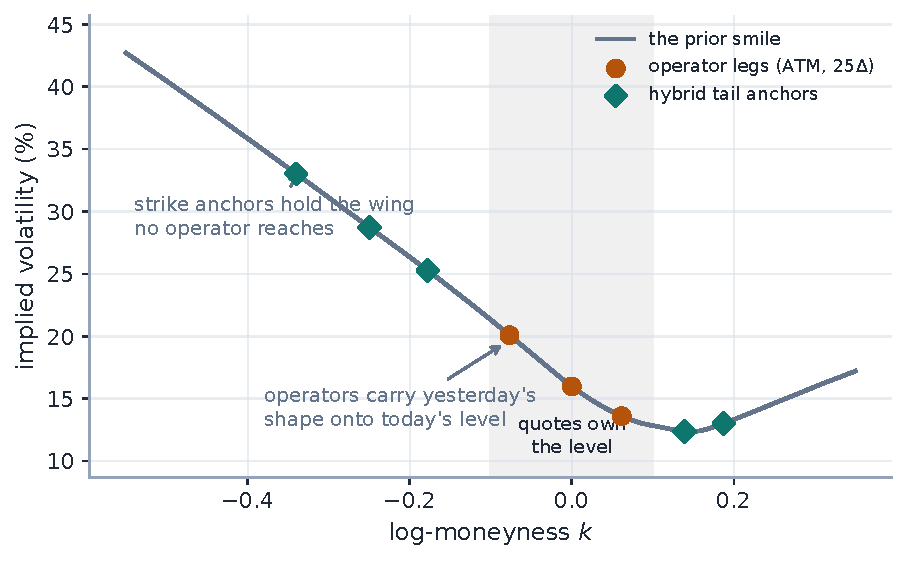
\includegraphics[width=0.9\textwidth]{fig_pfl_hybrid.pdf}
\caption{The hybrid division of labour on the running SPY node
(production leg and anchor placement).  Inside the quoted band every
gate closes and the data rules.  The $25\Delta$ operator legs carry
yesterday's shape onto today's level.  The tail anchors --- the
strike-gap machinery restricted to $\{\pfltaildeltas\}\Delta$ ---
hold the deep wing that no shape operator reaches.}
\label{fig:hybrid}
\end{figure}

\subsection{Two-pass activation}
\label{sec:twopass}

The sharpest observation precision is the \emph{realized} one --- how
well each operator is actually pinned by the fit --- which is a
chicken-and-egg with the fit the prior modifies.  The opt-in
\texttt{priorDataOnlyPrepass} resolves it exactly: fit once on data
alone, measure each operator's realized precision, refit with priors
active only on the genuinely under-observed coordinates.  It is the
most faithful no-damp behaviour at ${\sim}2\times$ cost per node; the
default single pass gates on quote support \eqref{eq:harmonic} with no
extra fit, and \cref{sec:blind} is the honest account of the
difference.

\begin{remark}[The filter already carries yesterday: auto-exclusion]
\label{rem:filter}
When the observation filter of Note~15 runs in \texttt{active} mode,
its Kalman prediction \emph{is} a prior on the ATM level and local
shape --- yesterday's state, propagated.  Anchoring the same
coordinates to the persisted prior as well would count yesterday
twice, so the resolver drops every overlapping builder --- operators,
factors, the near-ATM strike anchor --- and keeps exactly what the
filter state does not carry: the deep-tail strike anchor (for any
mode that had a calibration prior) and the graph's dark-node
baseline.  There is deliberately no knob; the exclusion is
test-locked (\cref{app:trace}).
\end{remark}

%======================================================================
\section{The prior must arrive in today's chart}
\label{sec:transport}

A prior fitted at yesterday's forward may not be compared to today's
smile raw --- the comparison itself must happen in today's
coordinates.  The stored prior's LQD backbone (the canonical persisted
object per expiry) is \emph{transported} to the current forward under
the active spot-dynamics regime of Note~12, with
$h=\log(F_{\mathrm{now}}/F_{\mathrm{prior}})$ the move; every
operator, factor and anchor target above is evaluated on the
transported smile.  The regime matters: under sticky-strike and
sticky-local-vol the same stored surface yields different transported
priors, and the persistence layer inherits whichever dynamics the
desk has chosen --- one more reason the prior's job is confined to
the flat directions, where the transport error has no data to
contradict it.

Provenance is part of the contract.  A snapshot stores, per expiry,
the LQD backbone plus the displayed-model parameters, forwards,
discounts and both clocks $(\tau,t)$; persistence is to the
\texttt{VolStore} database with history; and the active prior carries
a provenance source (\texttt{saved} / \texttt{15min} / \texttt{close}
/ \texttt{none}) and a per-ticker monotone version that busts the fit
cache --- a fetched prior can never silently coexist with fits made
under the old one.

%======================================================================
\section{Reading the gates: diagnostics}
\label{sec:diagnostics}

A prior that acts silently is a prior that gets blamed for
everything.  Persistence is therefore \emph{inspectable}: per node,
\texttt{GET /smiles/\{ticker\}/\{expiry\}/prior-diagnostics} answers
``is the prior pulling here, and how hard?''\ without reading code:

\begin{center}
\small
\begin{tabular}{p{0.28\textwidth}lp{0.50\textwidth}}
\toprule
Field & Type & Meaning\\
\midrule
\texttt{mode} / \texttt{active} & str / bool & Resolved mode; whether
any prior row is live on this node.\\
\texttt{operators[]} & list & One row per operator (active \emph{and}
gated-off).\\
\quad\texttt{operator} & str & ATM / RR25 / BF25 / VarSwap / factor
name.\\
\quad\texttt{priorValue} & float & The operator on the transported
prior.\\
\quad\texttt{obsPrecision} & float & Quote support
\eqref{eq:harmonic}.\\
\quad\texttt{requiredPrecision} & float & The gate threshold in
force.\\
\quad\texttt{gap} & float & The gate \eqref{eq:gate}: $0$ = off, $1$ =
full pull.\\
\quad\texttt{activeLambda} & float & The LSQ weight \eqref{eq:budget}
actually applied.\\
\texttt{varSwapPriorVol} / \texttt{varSwapWeight} & float & The
var-swap pull, if active.\\
\texttt{strikeAnchorCount} & int & Tail/strike anchors in force.\\
\bottomrule
\end{tabular}
\end{center}

The endpoint is best-effort --- it reports \emph{inactive} rather than
failing --- and drives the frontend persistence panel, whose table
shows the same gap and $\lambda$ columns.  \Cref{fig:activation} is
precisely this diagnostic rendered for the two shipped mechanisms.

%======================================================================
\section{What the proxy cannot see}
\label{sec:blind}

The gate is only as honest as its precision measure, and quote support
is a proxy, not the Fisher information.  Its blind spot has a sign:
the Gaussian kernel \eqref{eq:support} credits a leg with support from
quotes up to a bandwidth away, so support \emph{overstates}
identification just beyond the last quote --- precisely the region a
wing prior exists to protect.  The requirement $\pi_{\mathrm{req}}=1$
reads ``one effective quote suffices,'' and a dense at-the-money
cluster radiates enough kernel mass to satisfy it well outside the
band.

The running character measures the consequence.  On this node the
$25\Delta$ legs sit at $k=\pflkctwofivereal$ and
$k=\pflkptwofivereal$ --- inside the morning's quoted band --- so on
the dense morning every vol-operator gate closes (ATM
\pflgapdenseatm, RR25 \pflgapdenserr, BF25 \pflgapdensebf), and even
on a \pflnsparse-quote skeleton of the same band they stay closed;
only the var-swap probe, which reaches $1.4$ ATM standard deviations
into the wings, remains under-observed (gate \pflgapsparsevs\ on the
sparse morning).  The pure operator modes are therefore \emph{inert}
on liquid mornings: their rows never enter the optimizer, and the fit
is the prior-free fit --- which the temporal backtest of
\cref{sec:evidence} confirms at scale, showing exactly zero median
improvement for both pure basket modes.  The blind spot is why the
hybrid's tail anchor is not a refinement but a necessity: the
strike-gap deficit measures coverage \emph{against a desired span}
rather than radiated kernel mass, so it stays open in the wings that
support declares covered.

Two honest escapes exist.  The two-pass prepass
(\cref{sec:twopass}) replaces the proxy by the realized precision of
a data-only fit --- exact, at twice the cost, and opt-in.  And the
graph baseline of Note~14 prices the prior with the full vocabulary
\eqref{eq:factors} rather than support alone.  What ships as the
default is a calibrated compromise: proxy gates for the cheap common
case, deficit anchors where the proxy is blind, and the exact pass
available where a node justifies the spend.

%======================================================================
\section{Evidence}
\label{sec:evidence}

\subsection{Worked example: the running node, wing withheld}
\label{sec:example}

The protocol isolates the mechanism.  Take the running SPY node's
stored full-chain fit as the prior; keep only the \pflnthin\ quotes
with $|k|\le0.10$ as ``this morning''; withhold the other \pflnout\
real quotes; refit market-only and hybrid through the production
calibrator; score both against what was withheld.
\Cref{fig:spy} shows the result, and the two error numbers the
protocol was designed to separate: on the \emph{retained band} the
hybrid fit sits \pflspybandrms\ vol bp rms from the quotes --- the
prior has not damped the data it was given --- while on the
\emph{withheld wing} the market-only fit drifts \pflspywingmo\ vol bp
rms from the real quotes and the hybrid fit \pflspywinghy.  Because
the prior here is the same-day full fit, this is a mechanism test,
not a forecast: it certifies that the gates route yesterday's
information into exactly the coordinates the morning left dark.  The
forecast test --- where the prior is genuinely yesterday's --- is the
second case file below.

\begin{figure}[H]
\centering
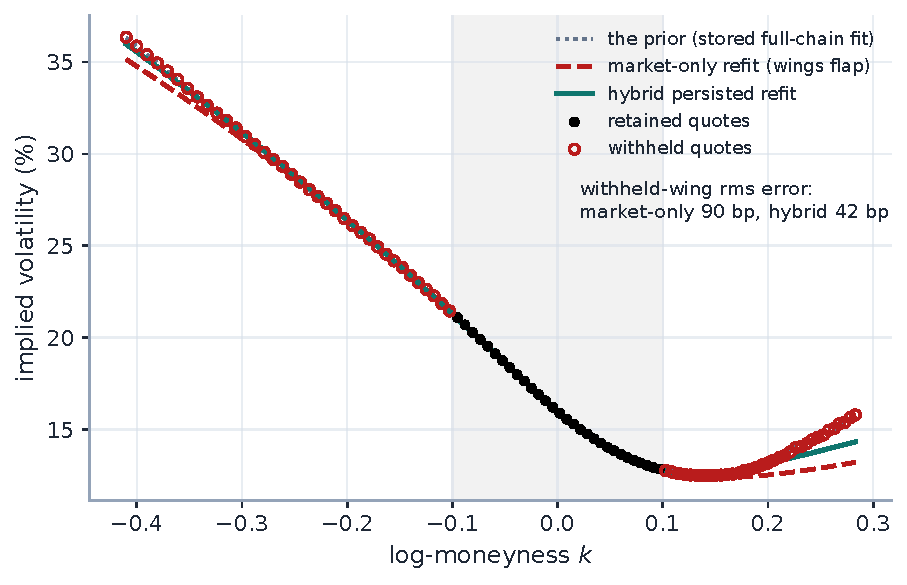
\includegraphics[width=0.9\textwidth]{fig_pfl_spy.pdf}
\caption{The hero protocol on the running SPY node (production fits
throughout).  Retained band (shaded): hybrid refit \pflspybandrms\
vol bp rms from the quotes --- no damping.  Withheld wing (open
markers): market-only \pflspywingmo\ vol bp rms, hybrid
\pflspywinghy\ --- the gap is filled with the prior's wing, visible
on the call side where the market-only fit misses the upturn
entirely.}
\label{fig:spy}
\end{figure}

\subsection{Case file: the jump the strike anchor damped}

\begin{example}[title={Case file: the jump the strike anchor damped}]
\textbf{Setup.}  The controlled experiment of \cref{fig:level}, which
is the runnable form of the production no-damp test: a $\tau=0.5$
node, an overnight level jump of \pfljump\ vol points with the shape
unchanged, today's quotes dense at the money and absent in the wings.
Operator prior (ATM/RR25/BF25) versus the strike-gap anchor, both
through the production calibrator.

\textbf{Failure mode.}  The strike anchor pins the unquoted wing to
yesterday's absolute wing vol --- after a level jump, the \emph{wrong}
wing: it undershoots today's true (lifted) wing and drags the nearby
smile with it.

\textbf{Diagnosis.}  \Cref{prop:nullspace}: per-strike price rows
penalize the level direction $\1$; RR/BF baskets are invariant under
it.  The gate also drops ATM automatically --- its quote support
exceeds the requirement --- so the operator target contains no row
that could damp the level (\cref{prop:nodamp} in action), and on this
market it drops BF25 too (\cref{rem:bfrr}), spending the whole budget
on the risk-reversal.

\textbf{Fix.}  Persist shape, not level: the operator rows carry
yesterday's skew onto today's level, and the wing is reconstructed as
``today's ATM $+$ yesterday's shape''.

\textbf{Verdict (test-locked, measured this build).}  At $k=-0.20$
the operator prior lands \pflopwingerrdeep\ vol points from the true
jumped wing; the strike anchor misses it by \pflsgwingerrdeep\ and
sits \pflsgoldgap\ from yesterday's curve --- still clinging.  The
operator and factor fits match the data-only ATM to \pflatmopgap\ and
\pflatmfacgap\ vol points: no damping.  \emph{Coordinates that
separate what the data measures from what it does not are not a
convenience; they are the difference between filling a gap and
fighting the tape.}
\end{example}

\subsection{Case file: the backtest that confirmed the default}

\begin{example}[title={Case file: the backtest that confirmed the
default}]
\textbf{Setup.}  The temporal harness over the stored August-2024
spike regime: for each asset and day pair $T{-}1\to T$, fit day
$T{-}1$'s full chain, freeze it as the active prior, thin day $T$ to
its ATM region, refit under each mode, and score the reconstructed
held-out moderate wing against day $T$'s true quotes; \texttt{off} is
the baseline.  \pflbtnodes\ node-days per mode; the stored artifact is
read, never re-run.

\textbf{Verdict.}  \Cref{fig:backtest}: the shipped \textbf{hybrid}
default reconstructs the held-out wing $\sim$\pflhybimpr\ vol bp
better than no prior at the median, winning \pflhybwin\% of node-days;
strike-gap is a close second (\pflsgimpr\ bp, \pflsgwin\%).  The
\emph{pure} basket modes do not beat \texttt{off} at the median ---
their win rates (\pflopwin\% and \pflfacwin\%) are below coin-flip and
their median improvement is exactly zero, the inertness of
\cref{sec:blind} at scale: with the wing dark but the band dense, the
proxy closes their gates and the fit is prior-free.  The recorded
knob sweep from the same campaign found neither the kernel bandwidth
nor the var-swap probe a productive lever; both stayed at their
defaults ($0.06$ and $1.4$ ATM standard deviations).

\textbf{Lesson.}  The backtest \emph{confirmed} rather than changed
the configuration: operators to avoid damping (previous case file),
the tail anchor to actually rebuild a dark wing.  \emph{Neither
component suffices alone; the composite does --- and the failure of
the pure modes is not noise but the measured shadow of the proxy's
blind spot.}
\end{example}

\begin{figure}[H]
\centering
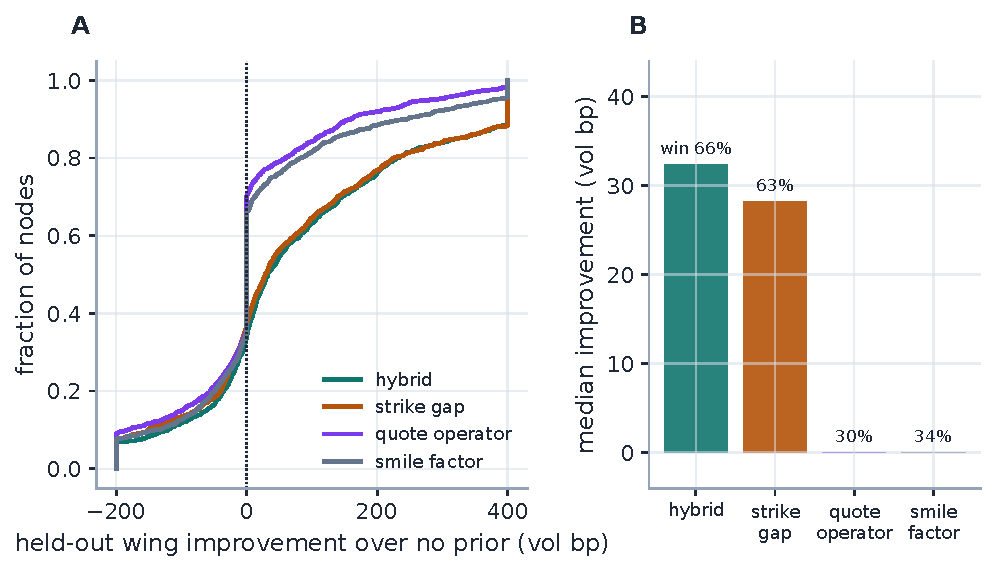
\includegraphics[width=\textwidth]{fig_pfl_backtest.pdf}
\caption{The stored temporal adjudication (\pflbtnodes\ node-days per
mode, spike regime; improvements clipped to $[-200,400]$ bp for
display).  A: distribution of held-out wing improvement over no
prior.  The vertical mass at zero for the pure basket modes is
inertness, not mediocrity: their gates close and the fit is
byte-identical to \texttt{off}.  B: medians with win rates --- hybrid
\pflhybimpr\ bp at \pflhybwin\%, strike-gap close behind, the pure
modes at zero.}
\label{fig:backtest}
\end{figure}

%======================================================================
\section{What is genuinely original here}
\label{sec:original}

The Bayesian framing is standard \cite{Gelman2013}; the contributions
are operational.  The \emph{activation gate} \eqref{eq:gate} turns
``do not damp the signal'' into one differentiable factor with a
provable dead zone (\cref{prop:nodamp}) --- gating where the
literature reaches for shrinkage.  The \emph{harmonic basket support}
\eqref{eq:harmonic} prices the identifiability of a combination
rather than of legs, with the dead-leg law and the RR/BF
factor-of-four (\cref{rem:bfrr}) as measurable consequences.  The
\emph{signed-basket coordinates} preserve exactly the level direction
per-leg persistence would damp (\cref{prop:nullspace}) --- the theorem
behind the measured case file, and the reform that cured the SVI/MCS
missing-prior asymmetry.  The \emph{shared vocabulary} keeps the
persistence gate and the graph baseline of Note~14 speaking one
identifiability language under golden re-export tests.  And the whole
framework is strictly additive: mode \texttt{off} is byte-identical
to a plain fit, so the prior can be adopted, audited and abandoned
per node without residue.

%======================================================================
\section{Limitations}
\label{sec:limits}

Where the guarantees stop.  \emph{The information model is diagonal}
(\cref{ass:diag}): support prices legs independently, ignoring the
covariance a smooth smile induces between neighbouring strikes, and
\texttt{priorOperatorCovarianceMode} accepts \texttt{full} but only
\texttt{diagonal} is implemented.  \emph{The proxy overstates
coverage near the band edge} (\cref{sec:blind}); the exact remedy
costs a second fit and is opt-in, and the shipped compensation is a
second mechanism, not a sharper measure.  \emph{One scalar
requirement governs all operators}: a per-operator
$\pi_{\mathrm{req}}$ schedule is declared in the design and not
implemented.  \emph{Strike anchors are wrong across level jumps} by
construction (\cref{fig:level}); the hybrid confines but does not
eliminate them --- across a jump, the deep tail is still pulled
toward yesterday's absolute prices.  \emph{The gate is heuristic
identifiability, not inference}: nothing estimates the actual
posterior variance of a persisted coordinate, and $\gamma$,
$\pi_{\mathrm{req}}$ and the budgets are set by judgment plus the
backtest, not by any optimality criterion.  \emph{Persistence is
per-node}: nothing here couples expiries or assets --- propagating a
lit node's innovation to a dark neighbour is the graph's job
(Note~14), which is why \texttt{graph\_only} exists.  A lecture that
sells a mechanism without drawing its boundary is an advertisement;
the boundary here is one honest sentence: \emph{the gate keeps
yesterday out of what today measured, to the accuracy of a kernel
proxy for ``measured''.}

\appendix
%======================================================================
\section{Hyperparameter atlas}
\label{app:atlas}

The only home for settings names: the body speaks mathematics, this
table speaks configuration.

\small
\setlength{\tabcolsep}{4pt}
\begin{longtable}{p{0.34\textwidth}p{0.15\textwidth}p{0.44\textwidth}}
\caption{Prior-persistence hyperparameters.}\label{tab:atlas}\\
\toprule Knob & Default & Role\\ \midrule
\endfirsthead \toprule Knob & Default & Role\\ \midrule \endhead
\multicolumn{3}{l}{\emph{Surfaced (options settings)}}\\ \midrule
\texttt{priorPersistenceMode} & \texttt{hybrid} & The mode selector
(\cref{sec:modes}); sole gate --- \texttt{autoLoadPrior} is retired
(migration only).\\
\texttt{priorAnchorWeightPct} & $50$ & Strike-gap budget (\% of summed
quote weights).\\
\texttt{priorAnchorDeltas} & $\{2,5,10,25,40\}\Delta$ & Delta
locations for strike anchors.\\
\texttt{priorOperatorSet} & ATM, RR25, BF25, VS & Operators to persist
(registry also knows RR10, BF10).\\
\texttt{priorOperatorStrengthPct} & $50$ & Operator budget.\\
\texttt{priorOperatorRequiredPrecision} & $1.0$ & Gate threshold
$\pi_{\mathrm{req}}$ (one scalar for all operators).\\
\texttt{priorOperatorGapExponent} $\gamma$ & $1.0$ & Gate sharpness.\\
\texttt{priorOperatorBandwidth} $b$ & $0.06$ & Quote-support kernel
bandwidth; also the factor stencil step.\\
\texttt{priorOperatorCovarianceMode} & \texttt{diagonal} & Declared
\texttt{diagonal}/\texttt{full}; only \texttt{diagonal} is
implemented.\\
\texttt{collarSign} & \texttt{call\_put} & RR orientation
($\pm(\sigma_c-\sigma_p)$).\\
\texttt{priorFactorSet} & ATM, skew, curv, VS & Factors to persist.\\
\texttt{priorFactorStrengthPct} & $50$ & Factor budget.\\
\texttt{priorTailAnchorStrengthPct} & $20$ & Hybrid deep-tail anchor
budget.\\
\texttt{priorDataOnlyPrepass} & \texttt{false} & Two-pass activation
(\cref{sec:twopass}).\\
\midrule
\multicolumn{3}{l}{\emph{Hidden (persistence path)}}\\ \midrule
\texttt{DEFAULT\_BANDWIDTH} & $0.06$ & Strike-gap KDE bandwidth.\\
\texttt{MAX\_INV\_VEGA\_RATIO} & $25$ & Cap on deep-wing
$1/\text{vega}$ amplification.\\
\texttt{\_VARSWAP\_PROBE\_STD} & $1.4$ & Var-swap coverage probe
half-width (ATM std units).\\
\texttt{\_WING\_MULT} & $3$ & Factor wing stencils at $\pm3b$.\\
\texttt{\_VOL\_TOL} (LV) & $0.01$ & Vol tolerance behind LV
basket/var-swap tolerances.\\
\midrule
\multicolumn{3}{l}{\emph{Hidden (shared vocabulary; consumed by the
graph baseline, Note~14)}}\\ \midrule
\texttt{RMS\_FLOOR} & $10^{-4}$ & Fit-quality precision floor (1 vol
bp).\\
\texttt{REF\_ATM\_QUOTES} & $8$ & Density credit saturation.\\
\texttt{MIN\_DENSITY\_FACTOR} & $0.15$ & Density credit floor.\\
\texttt{SPREAD\_HALF} & $0.05$ & Relative spread at which precision
halves.\\
\texttt{OBS/PRIOR} freshness half-lives & $3$ / $30$ d & Observation /
prior age decay.\\
\texttt{TRANSPORT\_SCALE} & $0.10$ & Transport-distance decay
scale.\\
\bottomrule
\end{longtable}
\normalsize

%======================================================================
\section{Performance notes}
\label{app:perf}

The prior blocks add a handful of constant-length residual rows ---
constant so the numeric Jacobian's sparsity never changes shape ---
and the single-pass gate is free: it reuses the quote locations the
fit already holds, and \eqref{eq:support}--\eqref{eq:budget} cost
$O(\#\text{quotes}\times\#\text{legs})$ kernel evaluations per node.
The two-pass prepass costs ${\sim}2\times$ per node and is opt-in.
Every prior knob bumps the options version (one refit on change), and
a fetched prior busts the fit cache through its monotone version
(\cref{sec:transport}) --- correctness spends, speed defaults.  Mode
\texttt{off} is byte-identical to a plain fit, so the entire feature
has zero cost when idle.  The temporal-backtest numbers of
\cref{sec:evidence} are read from the stored artifact
(\texttt{spike\_aug2024\_temporal\_prior.json}); no benchmark in this
note was re-timed.  Figures and macros were generated at commit
\texttt{\pflgencommit} on \pflgendate.

%======================================================================
\section{Traceability}
\label{app:trace}

\begingroup
\small
\setlength{\tabcolsep}{3pt}
\begin{longtable}{@{}p{0.28\textwidth}p{0.13\textwidth}p{0.27\textwidth}p{0.28\textwidth}@{}}
\caption{Claims in this note and the code/tests that lock them.}\\
\toprule Claim & Object & Code anchor & Test anchor\\ \midrule
\endfirsthead
\toprule Claim & Object & Code anchor & Test anchor\\ \midrule
\endhead
Gate: zero past requirement, monotone, $\gamma$ sharpens &
\cref{def:gate} &
\nolinkurl{calib/precision.py} &
\nolinkurl{test_precision_shared.py::test_gap_zero_when_well_observed},
\nolinkurl{::test_gap_monotone_and_gamma_sharpens}\\
No-damp / byte-identical off &
\cref{prop:nodamp} &
\nolinkurl{calib/prior.py}, \nolinkurl{api/prior_mode.py} &
\nolinkurl{test_prior_anchor.py::test_none_anchor_leaves_the_fit_byte_identical},
\nolinkurl{test_prior_parametric.py::test_none_arguments_are_noops}\\
Operator math (RR sign, BF convexity) &
\cref{def:operators} &
\nolinkurl{calib/operators.py} &
\nolinkurl{test_operators.py::test_risk_reversal_sign_and_collar},
\nolinkurl{::test_butterfly_positive_on_convex_smile}\\
Gate closes ATM on dense quotes, keeps wings &
\cref{prop:harmonic} &
\nolinkurl{calib/operators.py} &
\nolinkurl{test_operators.py::test_dense_atm_turns_off_atm_keeps_wings},
\nolinkurl{::test_full_coverage_returns_none}\\
Budget splits across open gates &
\eqref{eq:budget} &
\nolinkurl{calib/operators.py} &
\nolinkurl{test_operators.py::test_budget_splits_across_active_operators}\\
Factor stencils; hybrid tail below shallowest operator &
\cref{def:factors} &
\nolinkurl{calib/factors.py} &
\nolinkurl{test_prior_factors.py::test_factor_legs_stencils},
\nolinkurl{::test_hybrid_tail_deltas_below_shallowest_operator}\\
Strike-gap deficit weights; vega cap &
\eqref{eq:deficit} &
\nolinkurl{calib/prior.py} &
\nolinkurl{test_prior_anchor.py::test_prior_targets_gating},
\nolinkurl{::test_inv_vega_cap_bounds_tail_amplification}\\
Mode resolver; autoLoadPrior migration &
\cref{sec:modes} &
\nolinkurl{api/prior_mode.py}, \nolinkurl{api/settings_persist.py} &
\nolinkurl{test_prior_mode.py::test_resolver_flags_per_mode},
\nolinkurl{::test_migration_legacy_autoloadprior_on}\\
Observation-filter auto-exclusion &
\cref{rem:filter} &
\nolinkurl{api/prior_mode.py} &
\nolinkurl{test_filter_active.py::test_auto_exclusion_truth_table}\\
All models consume the prior (SVI/MCS asymmetry fixed) &
\cref{sec:coords} &
\nolinkurl{models/{lqd,svi_jw,sigmoid}/calibrate.py} &
\nolinkurl{test_prior_parametric.py::test_operator_prior_pulls_all_models_toward_prior_skew}\\
LV route emits signed baskets, not per-leg quotes &
\cref{prop:nullspace} &
\nolinkurl{api/prior_lv.py} &
\nolinkurl{test_prior_lv.py::test_rr_basket_is_a_signed_difference},
\nolinkurl{test_prior_factors.py::test_factor_lv_targets_are_baskets}\\
No-damp under a level jump (case file) &
\cref{sec:evidence} &
\nolinkurl{calib/operators.py} &
\nolinkurl{test_prior_nodamp.py::test_operator_prior_follows_level_and_reconstructs_jumped_wing}\\
Diagnostics endpoint &
\cref{sec:diagnostics} &
\nolinkurl{api/routers/smiles.py} &
\nolinkurl{test_prior_diagnostics.py::test_diagnostics_endpoint_ok}\\
Vocabulary shared with the graph (no drift) &
\cref{rem:notused} &
\nolinkurl{calib/precision.py}, \nolinkurl{graph/precision.py} &
\nolinkurl{test_precision_shared.py::test_graph_reexports_shared_factors},
\nolinkurl{::test_graph_design_point_unchanged}\\
Persistence round-trip; transported identity &
\cref{sec:transport} &
\nolinkurl{api/priors.py}, \nolinkurl{api/prior_transport.py} &
\nolinkurl{test_priors.py::test_priors_persist_across_restart},
\nolinkurl{::test_transported_prior_identity_and_shift}\\
\bottomrule
\end{longtable}
\endgroup

%======================================================================
\section{Reference implementation: the gated pipeline}
\label{app:ref}

The listing distills the full single-pass pipeline --- support,
basket precision, gate, budget split, and the scalar posterior a
gated row implements --- in numpy.  Executed against the production
builders on the case-file market and a $\gamma$ sweep of the gate,
the maximum discrepancy across gates, basket precisions and split
weights is at most \pflrefagree\ --- exact in double precision; the
formulas are the same arithmetic.

\begin{lstlisting}[caption={The gated pipeline (verified against
\texttt{calib/precision.py} and \texttt{calib/operators.py}) and the
scalar posterior a gated row implements.}]
def gate(obs, req, gamma=1.0):           # = activation_gap
    return np.clip(1 - obs/np.maximum(req, 1e-12), 0.0, 1.0)**gamma

def support(k_quotes, k_legs, b):        # quote count per leg
    z = (k_legs[:, None] - k_quotes[None, :]) / b
    return np.exp(-0.5*z*z).sum(axis=1)  # mean-1 weights

def basket_precision(c, s, eps=1e-9):    # the harmonic law
    nz = c != 0.0
    return 1.0 / np.sum(c[nz]**2 / (s[nz] + eps))

def split(budget, gaps):                 # zero gaps drop out
    return budget * gaps / gaps.sum()

def posterior(mu, lam, d, pi):           # lam = gated precision
    return (lam*mu + pi*d) / (lam + pi)
    # lam -> 0 (gate closed): posterior = d, no damping;
    # pi  -> 0 (data silent): posterior = mu, gap filled.
\end{lstlisting}

\begin{thebibliography}{9}
\bibitem{Gelman2013} A.~Gelman et al. \emph{Bayesian Data Analysis}.
CRC Press, 3rd ed., 2013.
\bibitem{Gatheral2006} J.~Gatheral. \emph{The Volatility Surface}.
Wiley, 2006.
\bibitem{LehmannCasella1998} E.~Lehmann and G.~Casella. \emph{Theory
of Point Estimation}. Springer, 2nd ed., 1998.
\bibitem{Tikhonov1977} A.~Tikhonov and V.~Arsenin. \emph{Solutions of
Ill-Posed Problems}. Winston, 1977.
\end{thebibliography}

\end{document}
